\textbf{Pour cette première partie, aucune justification n'est demandée et une seule réponse est possible par question. Pour chaque question, reportez son numéro sur votre copie et indiquez votre réponse.}

\subsubsection*{Question 1}
Un article coûte 400 euros. Le prix augmente de 20\%. Le nouveau prix est

\textbf{a.} 420 euros \hfill \textbf{b.} 480 euros \hfill \textbf{c.} 500 euros \hfill \textbf{d.} 320 euros

\subsubsection*{Question 2}
Un sac coûte 130 euros. Le prix baisse de 10\%. Le nouveau prix est

\textbf{a.} $130 \times 0,1$ \hfill \textbf{b.} $130 \times \left(-\dfrac{10}{100}\right)$ \hfill \textbf{c.} $130 \times \left(1 + \dfrac{10}{100}\right)$ \hfill \textbf{d.} $130 \times 0,9$

\subsubsection*{Question 3}
Le prix d'un article est noté $P$. Il connaît deux augmentations de 20\%. \\
Le prix après ces augmentations est

\textbf{a.} $P \times \left(1 + \left(\dfrac{20}{100}\right)^2\right)$ \hfill \textbf{b.} $P \times 1,40$ \hfill \textbf{c.} $\dfrac{P}{1,44}$ \hfill \textbf{d.} $P \times 1,2^2$

\subsubsection*{Question 4}
Lors d'une élection, le quart des électeurs a voté pour A, 20\% a voté pour B, un tiers a voté pour C, et le reste a voté pour D. \\
Le candidat ayant recueilli le \underline{moins} de votes est

\textbf{a.} A \hfill \textbf{b.} B \hfill \textbf{c.} C \hfill \textbf{d.} D

\subsubsection*{Question 5}
On considère $A = \dfrac{2}{1 - \dfrac{2}{3}}$. On a

\textbf{a.} $A = -1$ \hfill \textbf{b.} $A = \dfrac{2}{3}$ \hfill \textbf{c.} $A = 6$ \hfill \textbf{d.} $A = 9$

\subsubsection*{Question 6}
On considère $A = \dfrac{1}{100} + \dfrac{1}{1\,000}$. On a

\textbf{a.} $A = 100,001$ \hfill \textbf{b.} $A = \dfrac{2}{100\,000}$ \hfill \textbf{c.} $A = 0,11$ \hfill \textbf{d.} $A = 0,011$

\subsubsection*{Question 7}
Une durée de 75 minutes correspond à

\textbf{a.} 1,15 heure \hfill \textbf{b.} 1,25 heure \hfill \textbf{c.} 0,75 heure \hfill \textbf{d.} 1,4 heure

\subsubsection*{Question 8}
$10^{30} + 10^{-30}$ est environ égal à

\textbf{a.} $10^0$ \hfill \textbf{b.} 0 \hfill \textbf{c.} $10^{30}$ \hfill \textbf{d.} $20^{30}$

\subsubsection*{Question 9}
La seule droite pouvant correspondre à l'équation $y = -2x + 5$ est

\begin{minipage}[t]{0.24\textwidth}
\begin{center}
\textbf{a.} la droite $D_1$

\medskip

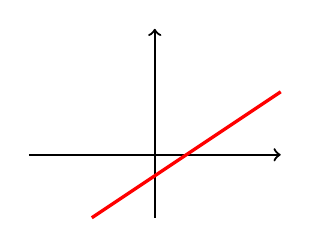
\begin{tikzpicture}[scale=0.8]
\draw[thick, ->] (-2,0) -- (2,0);
\draw[thick, ->] (0,-1) -- (0,2);
\draw[very thick, color=red] (-1,-1) -- (2,1);
\end{tikzpicture}
\end{center}
\end{minipage}
\hfill
\begin{minipage}[t]{0.24\textwidth}
\begin{center}
\textbf{b.} la droite $D_2$

\medskip

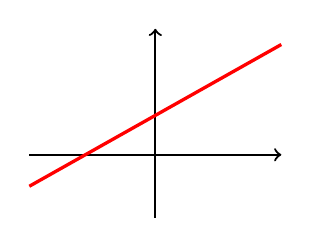
\begin{tikzpicture}[scale=0.8]
\draw[thick, ->] (-2,0) -- (2,0);
\draw[thick, ->] (0,-1) -- (0,2);
\draw[very thick, color=red] (-2,-0.5) -- (2,1.75);
\end{tikzpicture}
\end{center}
\end{minipage}
\hfill
\begin{minipage}[t]{0.24\textwidth}
\begin{center}
\textbf{c.} la droite $D_3$

\medskip

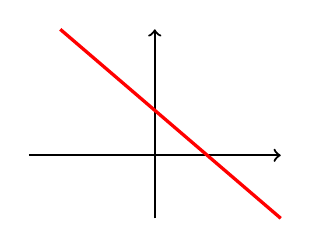
\begin{tikzpicture}[scale=0.8]
\draw[thick, ->] (-2,0) -- (2,0);
\draw[thick, ->] (0,-1) -- (0,2);
\draw[very thick, color=red] (-1.5,2) -- (2,-1);
\end{tikzpicture}
\end{center}
\end{minipage}
\hfill
\begin{minipage}[t]{0.24\textwidth}
\begin{center}
\textbf{d.} la droite $D_4$

\medskip

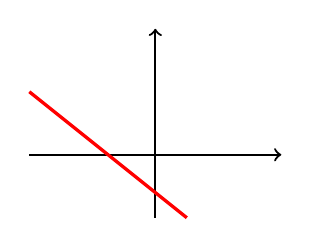
\begin{tikzpicture}[scale=0.8]
\draw[thick, ->] (-2,0) -- (2,0);
\draw[thick, ->] (0,-1) -- (0,2);
\draw[very thick, color=red] (-2,1) -- (0.5,-1);
\end{tikzpicture}
\end{center}
\end{minipage}

\subsubsection*{Question 10}
La solution de l'équation $3x = 0$ est

\textbf{a.} $x = -3$ \hfill \textbf{b.} $x = \dfrac{1}{3}$ \hfill \textbf{c.} $x = -\dfrac{1}{3}$ \hfill \textbf{d.} $x = 0$

\subsubsection*{Question 11}
La solution de l'équation $\dfrac{144}{x} = 9$ est

\textbf{a.} $x = 144 \times 9$ \hfill \textbf{b.} $x = \dfrac{9}{144}$ \hfill \textbf{c.} $x = \dfrac{144}{9}$ \hfill \textbf{d.} $x = -16$

\subsubsection*{Question 12}
Voici les notes sur vingt obtenues par un élève en mathématiques :

\begin{center}
\begin{tabular}{|c|c|c|c|c|}
\hline
Note & 10 & 13 & 12 & $x$ \\
\hline
Coefficient & 1 & 1 & 1 & 2 \\
\hline
\end{tabular}
\end{center}

On cherche ce que doit valoir $x$ pour que la moyenne de l'élève soit égale à 15.

\textbf{a.} $x = 20$ \hfill \textbf{b.} $x = 18$

\textbf{c.} $x = 15$ \hfill \textbf{d.} Impossible : il faudrait une note strictement supérieure à vingt.
